\chapter{Poisson denoising}
\label{ch_denoising}

\markright{Poisson denoising}

\section{MS-VST + IUWT}

Under the hypothesis of homogeneous Poisson intensity, the stabilized wavelet coefficients $d_j$ behave like centered Gaussian variables of standard deviation $\sigma_{(j)}$. We can detect significant coefficients with binary hypothesis testing as in Gaussian denoising.

Under the null hypothesis $\mathcal{H}_0$ of homogeneous Poisson intensity, the distribution of the stabilized wavelet coefficient $d_j[k]$ at scale $j$ and location index $k$ can be written as:
\begin{equation}
\label{ }
p(d_j[k]) = \frac{1}{\sqrt{2\pi}\sigma_j}\exp(-d_j[k]^2 / 2 \sigma_j^2) .
\end{equation}

The rejection of the hypothesis $\mathcal{H}_0$ depends on the double-sided p-value:
\begin{equation}
\label{ }
p_j[k] = 2 \frac{1}{\sqrt{2\pi}\sigma_j}\int_{|d_j[k]|}^{+\infty} \exp(-x^2 / 2 \sigma_j^2) dx .
\end{equation}

Consequently, to accept or reject $\mathcal{H}_0$, we compare each $|d_j[k]|$ with a critical threshold $\kappa \sigma_j$, $\kappa= 3,4 \text{ or } 5$ corresponding respectively to significance levels. This amounts to deciding that:
\begin{itemize}
  \item if $|d_j[k]| \geqslant  \kappa \sigma_j$, $d_j[k]$ is significant.
  \item if $|d_j[k]| < \kappa \sigma_j$, $d_j[k]$ is not significant.
\end{itemize}

Then we have to invert the MS-VSTS scheme to reconstruct the estimate. However, although the direct inversion is possible (Eq. (\ref{eq30})), it can not guarantee a positive intensity estimate, while the Poisson intensity is always nonnegative. A positivity projection can be applied, but important structures could be lost in the estimate. To tackle this problem, we reformulate the reconstruction as a convex optimisation problem and solve it iteratively with an algorithm based on Hybrid Steepest Descent (HSD)~\citep{wave:yamada01}.

We define the multiresolution support $\mathcal{M}$, which is determined by the set of detected significant coefficients after hypothesis testing:
\begin{equation}
\label{eq33}
\mathcal{M} := \{ (j,k) | \text{if } d_j[k] \text{ is declared significant} \} .
\end{equation}

We formulate the reconstruction problem as a convex constrained minimization problem:

\begin{equation}
\label{eq34}
\begin{split}
\text{Arg} \min_{\mathbf{X}} \| \mathbf{ \Phi}^{T}\mathbf{X}\|_1,
\text{s.t.} \\ \: \left\{\begin{array}{c}\mathbf{X} \geqslant 0 , \\\forall (j,k)\in \mathcal{M},      (\mathbf{ \Phi}^{T}\mathbf{X})_j[k]=(\mathbf{ \Phi}^{T}\mathbf{Y})_j[k] , \end{array}\right.
\end{split}
\end{equation}
where $\mathbf{\Phi}$ denotes the IUWT synthesis operator.

This problem is solved with the following iterative scheme: the image is initialised by $\mathbf{X}^{(0)} = 0$, and the iteration scheme is, for $n=0$ to $N_{\max}-1$:


\begin{eqnarray}
\tilde{\mathbf{X}} &=& P_{+}[\mathbf{ X}^{(n)} + \mathbf{ \Phi} P_{\mathcal{M}} \mathbf{ \Phi}^{T} (\mathbf{ Y} - \mathbf{ X}^{(n)})] \\
\mathbf{X}^{(n+1)} &=& \mathbf{ \Phi}\text{ST}_{\lambda_n}[\mathbf{ \Phi}^{T}\tilde{\mathbf{X}}]
\end{eqnarray}
where $P_{+}$ denotes the projection on the positive orthant, $P_{\mathcal{M}}$ denotes the projection on the multiresolution support $\mathcal{M}$:
\begin{equation}
P_{\mathcal{M}}d_j[k] = \left\{\begin{array}{cc} d_j[k] & \text{if} \  (j,k) \in \mathcal{M} , \\0 & \text{otherwise} \end{array} . \right.
\end{equation}
and $\text{ST}_{\lambda_n}$ the soft-thresholding with threshold $\lambda_n$:
\begin{equation}
\text{ST}_{\lambda_n} [d] = \left\{\begin{array}{cc} \mathrm{sign}(d)(|d| - \lambda_n) & \text{if} \ |d| \geqslant \lambda_n , \\0 & \text{otherwise} \end{array} . \right.
\end{equation}
We chose a decreasing threshold $\lambda_n = \frac{N_{\max} - n}{N_{\max} - 1},n=1,2,\cdots,N_{\max}$.

The final estimate of the Poisson intensity is: $\hat{\mathbf{\Lambda}} = \mathbf{X}^{(N_{\max})}$. Algorithm~\ref{alg1} summarizes the main steps of the MS-VSTS + IUWT denoising algorithm.



\begin{algorithm}[!h]
\caption{MS-VSTS + IUWT Denoising}
\label{alg1}
\begin{algorithmic}[1]
\REQUIRE $\quad$ data $a_0:=\mathbf{Y}$, number of iterations $N_{\max}$, threshold $\kappa$ \\
\underline{\emph{\textbf{Detection}}} \\
\FOR{$j=1$ to $J$}
\STATE Compute $a_j$ and $d_j$ using (\ref{eq27}).
\STATE Hard threshold $|d_j[k]|$ with threshold $\kappa \sigma_j$ and update $\mathcal{M}$.
\ENDFOR \\
\underline{\emph{\textbf{Estimation}}} \\
\STATE Initialize $\mathbf{X}^{(0)}=0$, $\lambda_0 = 1$.
\FOR{$n=0$ to $N_{\max}-1$}
\STATE $\tilde{\mathbf{X}}= P_{+}[\mathbf{ X}^{(n)} + \mathbf{ \Phi} P_{\mathcal{M}} \mathbf{ \Phi}^{T} (\mathbf{ Y} - \mathbf{ X}^{(n)})]$.
\STATE $\mathbf{X}^{(n+1)} = \mathbf{ \Phi}\text{ST}_{\lambda_n}[\mathbf{ \Phi}^{T}\tilde{\mathbf{X}}]$.
\STATE $\lambda_{n+1} = \frac{N_{\max} - (n+1)}{N_{\max} - 1}$.
\ENDFOR
\STATE Get the estimate $\hat{\mathbf{\Lambda}} = \mathbf{X}^{(N_{\max})}$.

\end{algorithmic}
\end{algorithm}


\section{Multi-resolution support adaptation}

When two sources are too close, the less intense source may not be detected because of the negative wavelet coefficients of the brightest source. To avoid such a drawback, we may update the multi-resolution support at each iteration. The idea is to withdraw the detected sources and to make a detection on the remaining residual, so as to detect the sources which may have been missed at the first detection.


At each iteration $n$, we compute the MS-VSTS of $\mathbf{X}^{(n)}$. We denote $d^{(n)}_j[k]$ the stabilised coefficients of $\mathbf{X}^{(n)}$. We make a hard thresholding on $(d_j[k]-d^{(n)}_j[k])$ with the same thresholds as in the detection step. Significant coefficients are added to the multiresolution support $\mathcal{M}$.

\begin{algorithm}
\caption{MS-VSTS + IUWT Denoising + Multiresolution Support Adaptation}
\label{alg4}
\begin{algorithmic}[1]
\REQUIRE $\quad$ data $a_0:=\mathbf{Y}$, number of iterations $N_{\max}$, threshold $\kappa$ \\
\underline{\emph{\textbf{Detection}}} \\
\FOR{$j=1$ to $J$}
\STATE Compute $a_j$ and $d_j$ using (\ref{eq27}).
\STATE Hard threshold $|d_j[k]|$ with threshold $\kappa \sigma_j$ and update $\mathcal{M}$.
\ENDFOR \\
\underline{\emph{\textbf{Estimation}}} \\
\STATE Initialize $\mathbf{X}^{(0)}=0$, $\lambda_0 = 1$.
\FOR{$n=0$ to $N_{\max}-1$}
\STATE $\tilde{\mathbf{X}}= P_{+}[\mathbf{ X}^{(n)} + \mathbf{ \Phi} P_{\mathcal{M}} \mathbf{ \Phi}^{T} (\mathbf{ Y} - \mathbf{ X}^{(n)})]$.
\STATE $\mathbf{X}^{(n+1)} = \mathbf{ \Phi}\text{ST}_{\lambda_n}[\mathbf{ \Phi}^{T}\tilde{\mathbf{X}}]$.
\STATE Compute the MS-VSTS on  $\mathbf{X}^{(n)}$ to get the stabilised coeffcients $d^{(n)}_j$.
\STATE Hard threshold $|d_j[k]-d^{(n)}_j[k]|$ and update $\mathcal{M}$.
\STATE $\lambda_{n+1} = \frac{N_{\max} - (n+1)}{N_{\max} - 1}$.
\ENDFOR
\STATE Get the estimate $\hat{\mathbf{\Lambda}} = \mathbf{X}^{(N_{\max})}$.

\end{algorithmic}
\end{algorithm}

The main steps of the algorithm are summarized in Algorithm~\ref{alg4}. In practice, we use Algorithm~\ref{alg4} instead of Algorithm~\ref{alg1} in our experiments.

\section{MS-VST + Curvelets}

Insignificant coefficients are zeroed by using the same hypothesis testing framework as in the wavelet scale. At each wavelet scale $j$ and ridgelet band $k$, we make a hard thresholding on curvelet coefficients with threshold $\kappa \sigma_{j,k}$, $\kappa= 3,4 \text{ or } 5$. Finally, a direct reconstruction can be performed by first inverting the local ridgelet transforms and then inverting the MS-VST + IUWT~(Equation~(\ref{eq30})). An iterative reconstruction may also be performed.

Algorithm~\ref{algcurv} summarizes the  main steps of the MS-VSTS + Curvelets denoising algorithm.

\begin{algorithm}
\caption{MS-VSTS + Curvelets Denoising}
\label{algcurv}
\begin{algorithmic}[1]
\STATE Apply the MS-VST + IUWT with $J$ scales to get the stabilized wavelet subbands $d_j$.
\STATE Set $B_1 = B_{\min}$.
\FOR{$j=1$ to $J$}
\STATE Partition the subband $d_j$ with blocks of side-length $B_j$ and apply the digital ridgelet transform to each block to obtain the stabilized curvelets coefficients.
\IF {$j$ modulo $2=1$}
\STATE $B_{j+1} = 2 B_j$
\ELSE
\STATE $B_{j+1} =  B_j$
\ENDIF \\
\STATE HTs on the stabilized curvelet coefficients.
\ENDFOR \\
\STATE Invert the ridgelet transform in each block before inverting the MS-VST + IUWT.

\end{algorithmic}
\end{algorithm}


\section{Experiments}

The method was tested on simulated Fermi data. The simulated data are the sum of a Milky Way diffuse background model and 1000 gamma ray point sources. We based our Galactic diffuse emission model intensity on the model $gll\_iem\_v02$ obtained at the Fermi Science Support Center~\citep{Models}
. This model results from a fit of the LAT photons with various gas templates as well as inverse Compton in several energy bands. We used a realistic point-spread function for the sources, based on Monte Carlo simulations of the LAT and accelerator tests, that scale approximately as $0.8(E/1GeV)^{-0.8}$ degrees. The position of the 205 brightest sources were taken from the Fermi 3-month source list~\citep{Abdo}. The position of the 795 remaining sources follow the LAT 1-year Point Source Catalog~\citep{Catalog}
  sources distribution: each simulated source was randomly sorted in a box of $\Delta$l=5$^o$ and $\Delta$b=1$^o$ around a LAT 1-year catalog source. We simulated each source assuming a power-law dependence with its spectral index given by the 3-month source list and the first year catalog. We used an exposure of $3.10^{10} s.cm^2$ corresponding approximatively to one year of Fermi all-sky survey around 1 GeV. The simulated counts map shown here correspond to photons energy from 150 MeV to 20 GeV.


Fig.~\ref{rechsd} compares the result of denoising with MS-VST + IUWT (Algorithm~\ref{alg1}), MS-VST + curvelets (Algorithm~\ref{algcurv}) and Anscombe VST + wavelet shrinkage on a simulated Fermi map. Fig.~\ref{recface} shows one HEALPix face of the results. 
As expected from theory, the Anscombe method produces poor results to  denoise Fermi data, because the underlyning intensity is too weak. 
Both wavelet and curvelet denoising on the sphere  perform much better. 
For this application, wavelets are slightly better than curvelets ($SNR_{wavelets} = 65.8 dB$, $SNR_{curvelets} = 37.3 dB$, $SNR (dB) = 20 \log (\sigma_{signal} / \sigma_{noise})$). As this image contains many point sources, thisresult is expected. Indeed wavelet are better than curvelets to represent isotropic objects.

\begin{figure}[htb]
\centering{
\hbox{
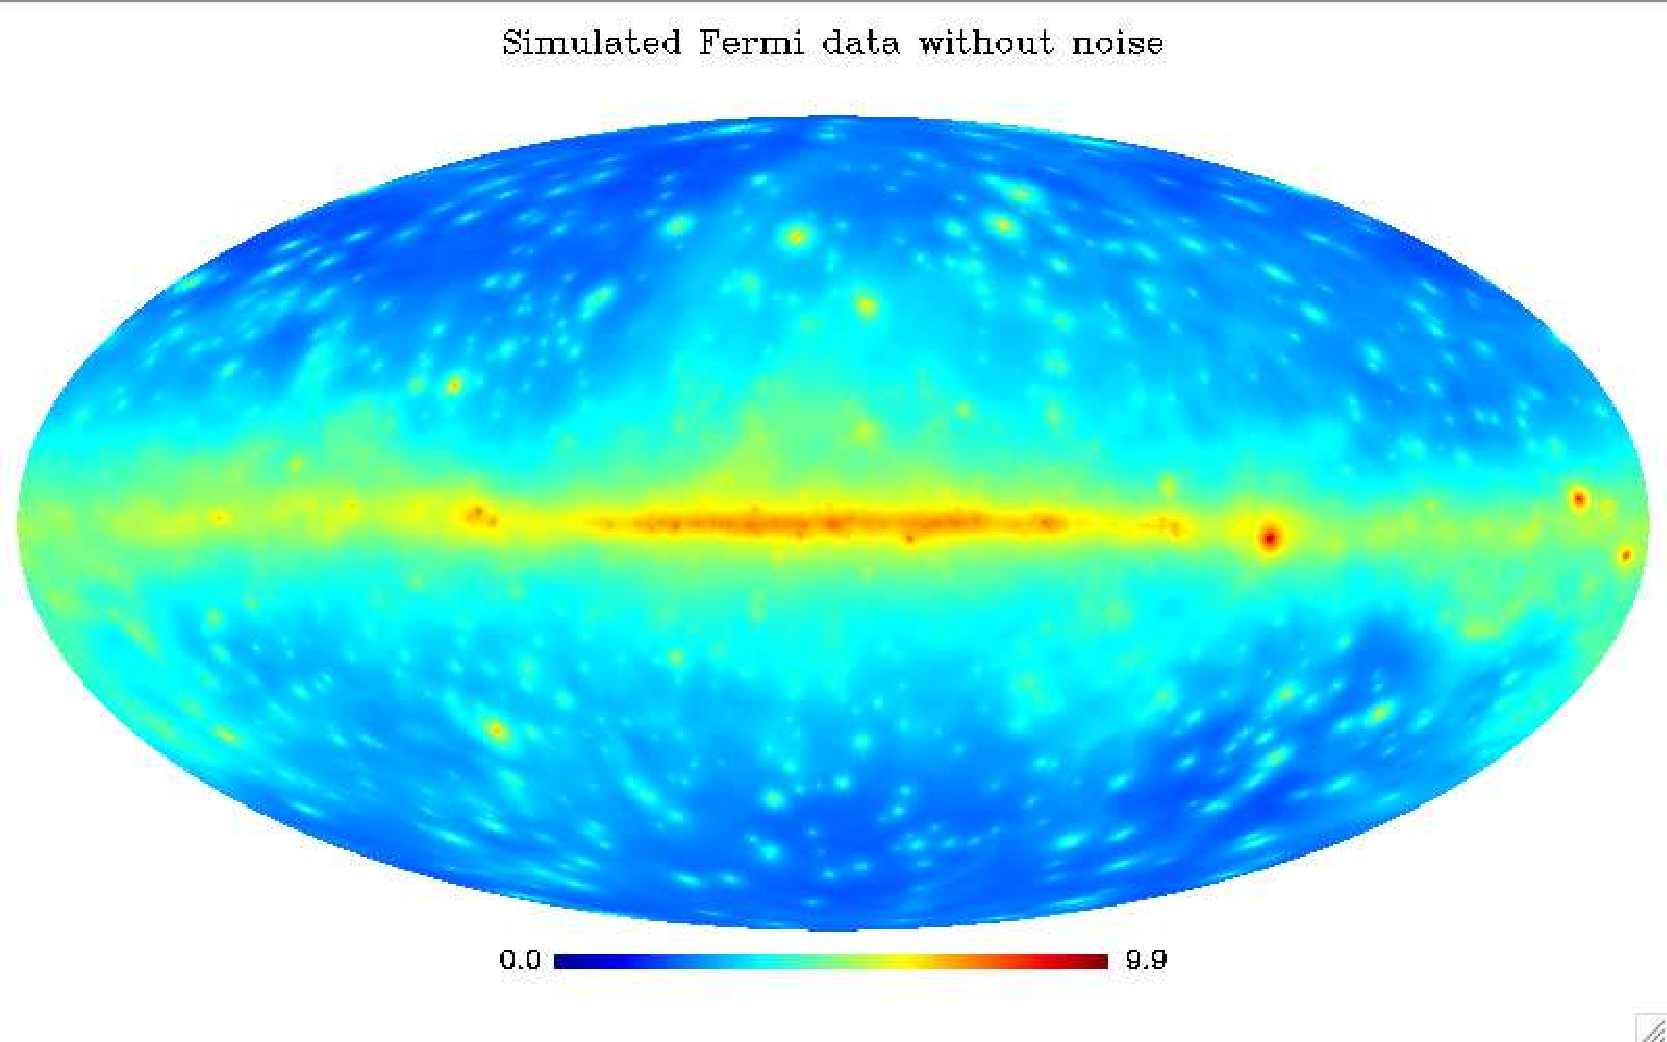
\includegraphics[width=3in,height=2.4in]{13822fg10.pdf}  
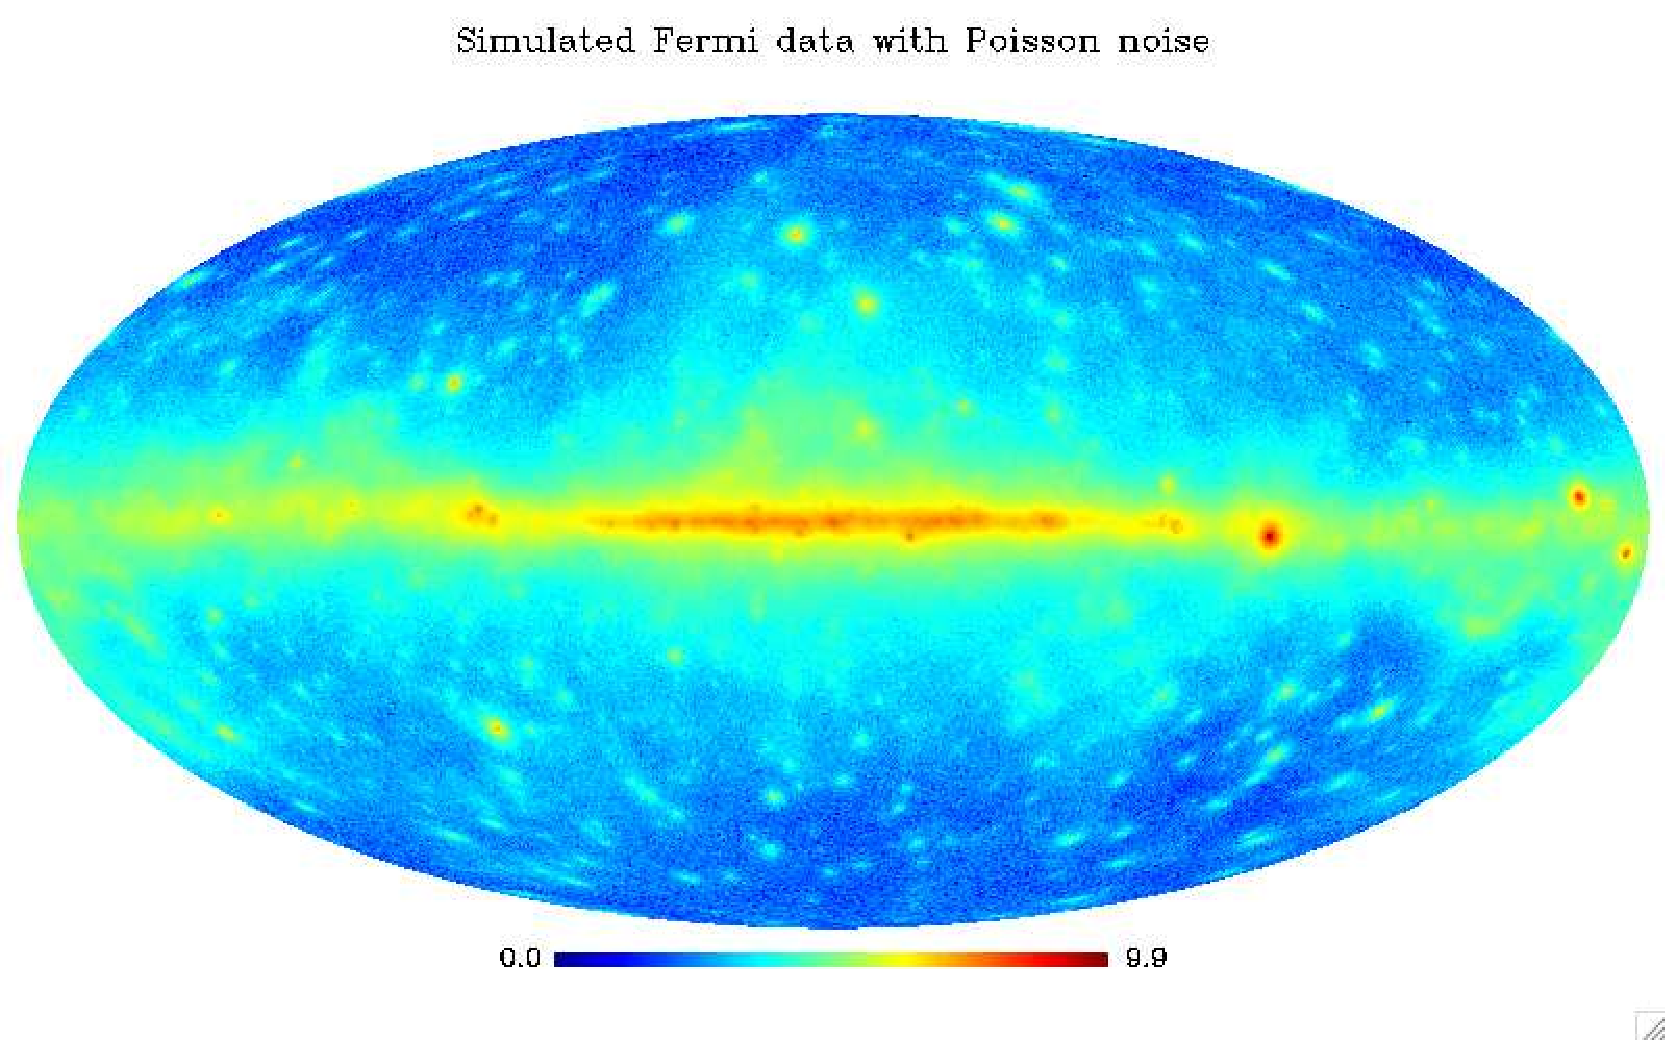
\includegraphics[width=3in,height=2.4in]{13822fg11.pdf}} 
\hbox{
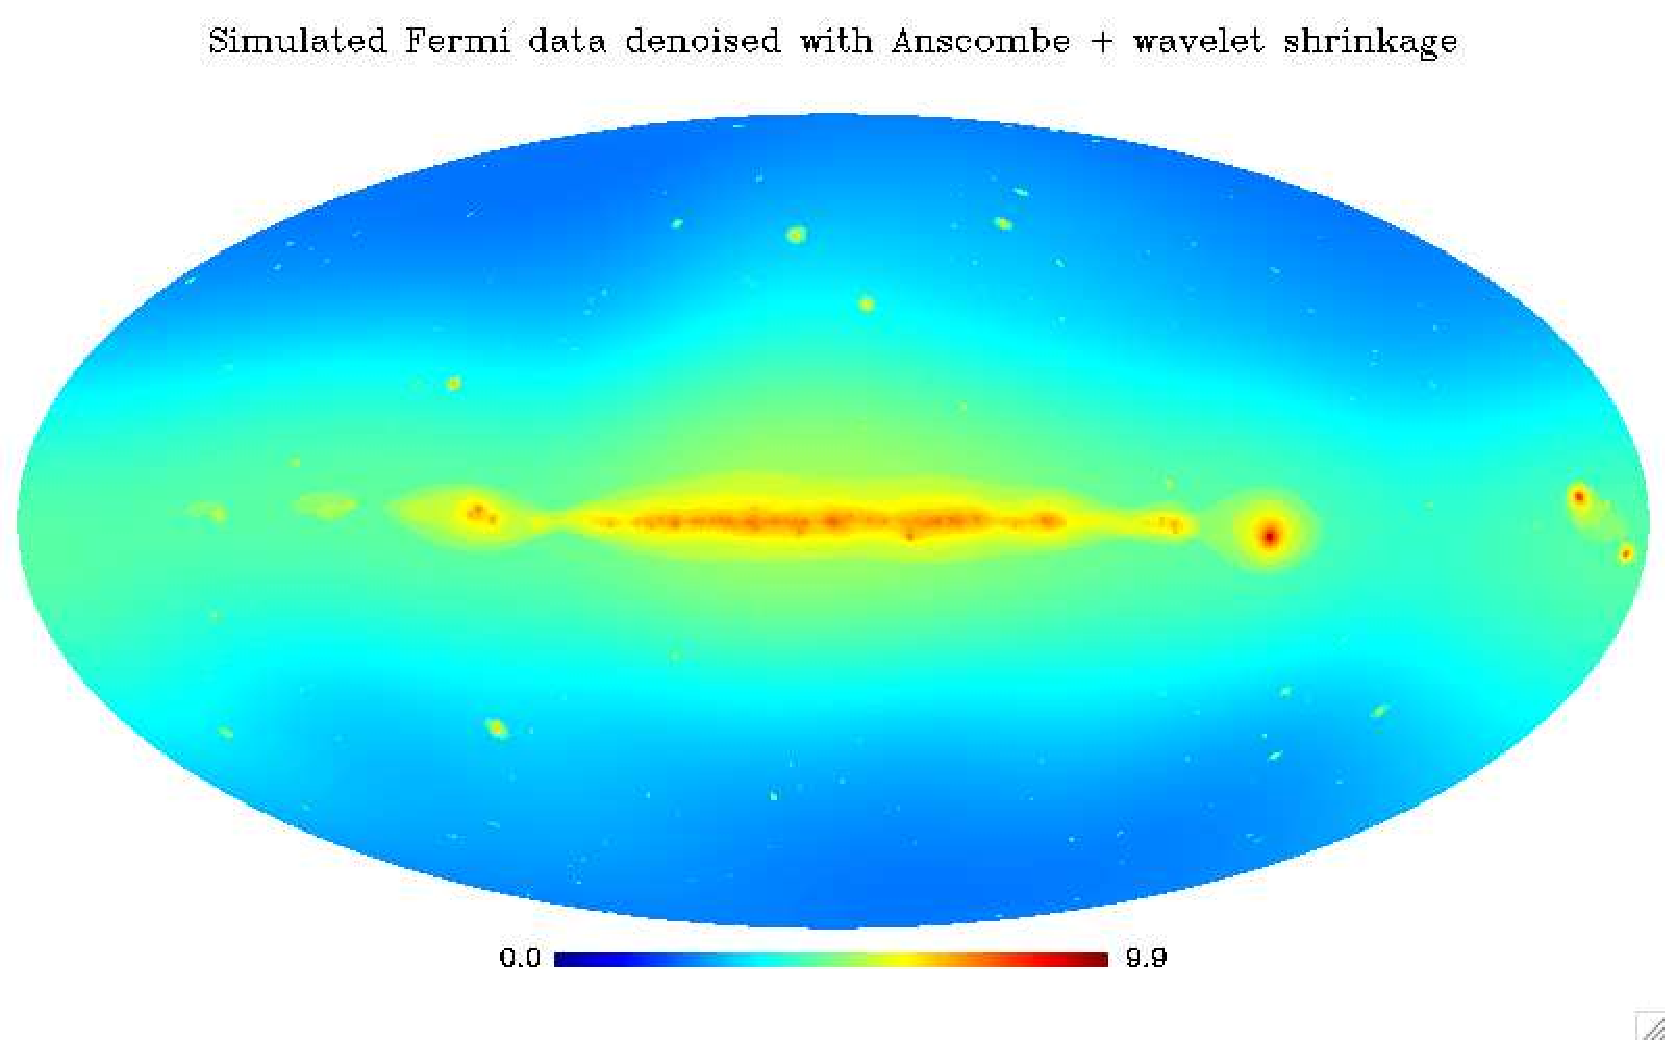
\includegraphics[width=3in,height=2.4in]{13822fg12.pdf} 
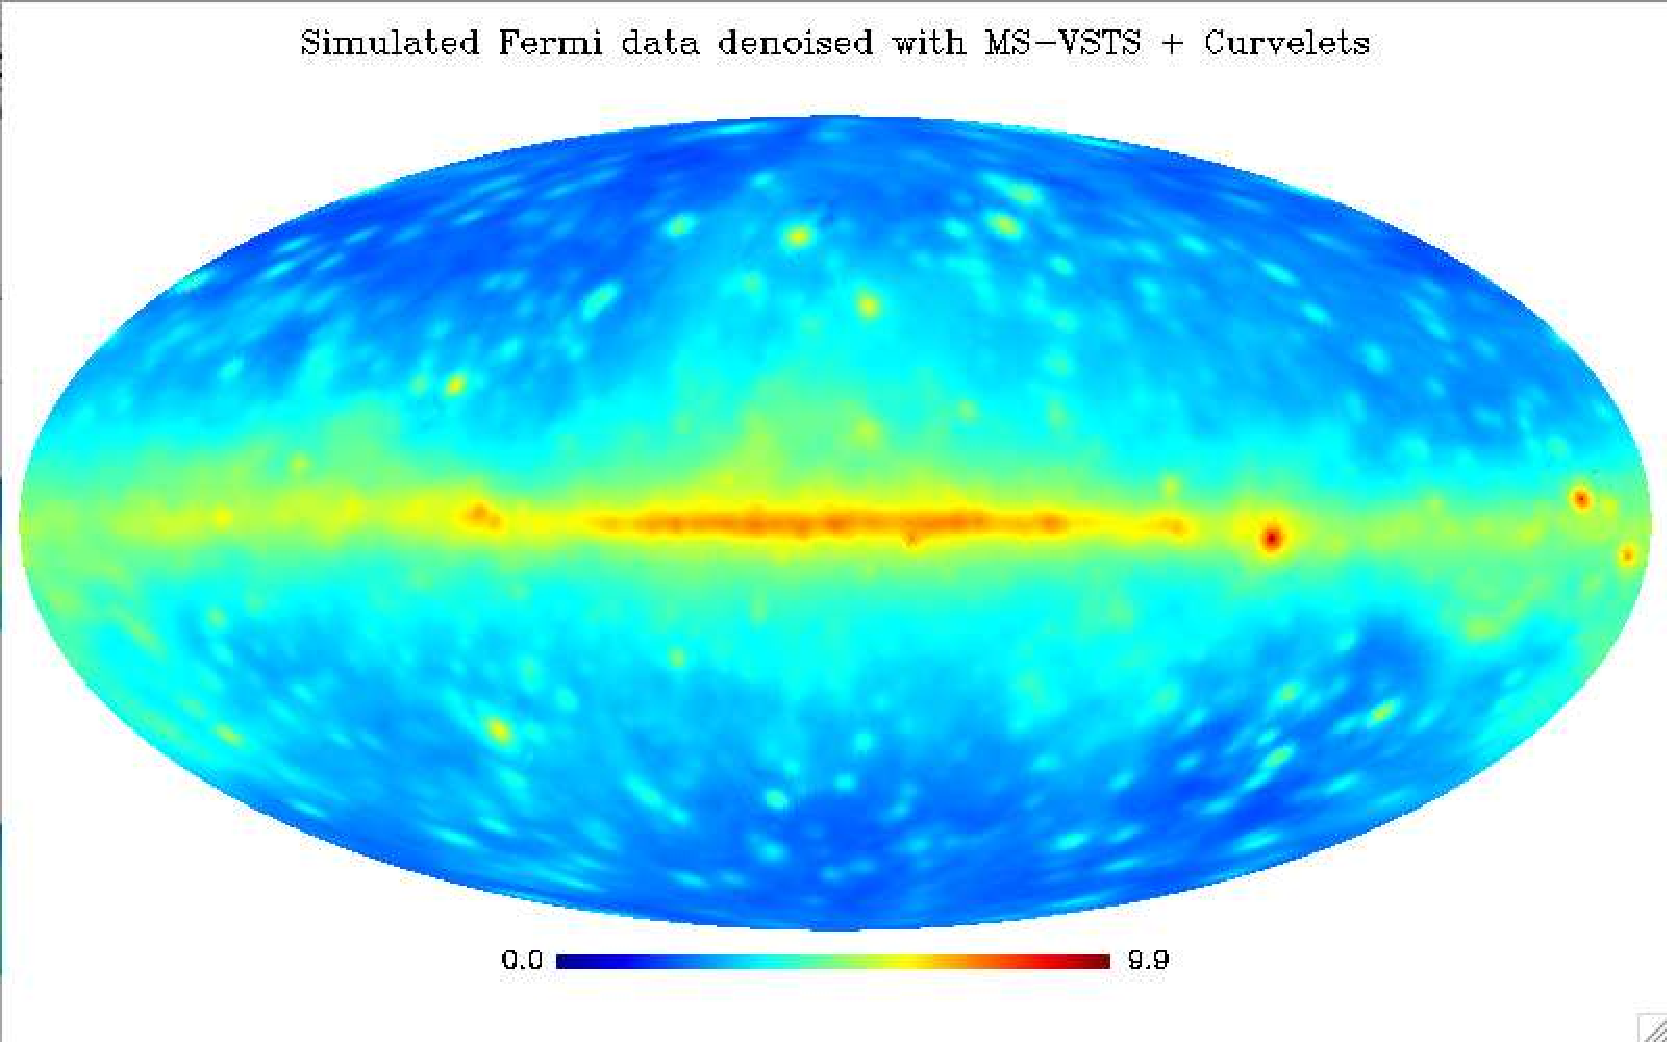
\includegraphics[width=3in,height=2.4in]{13822fg13.pdf}}
\hbox{
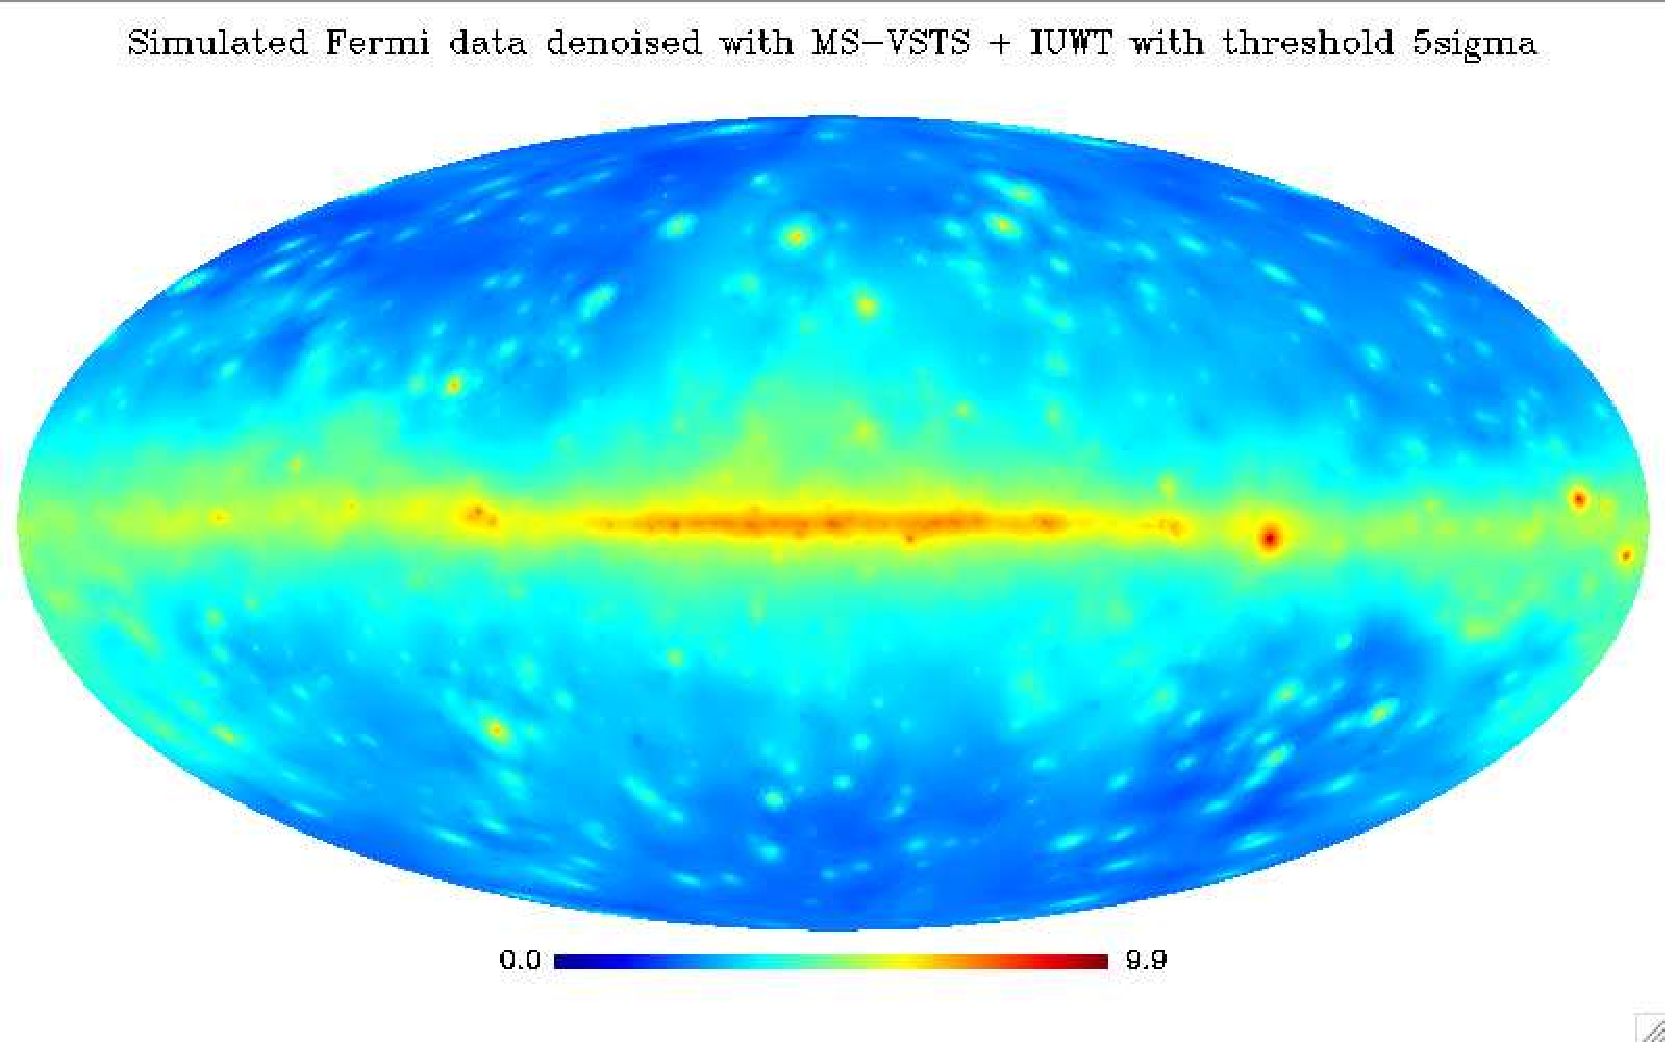
\includegraphics[width=3in,height=2.4in]{13822fg14.pdf} 
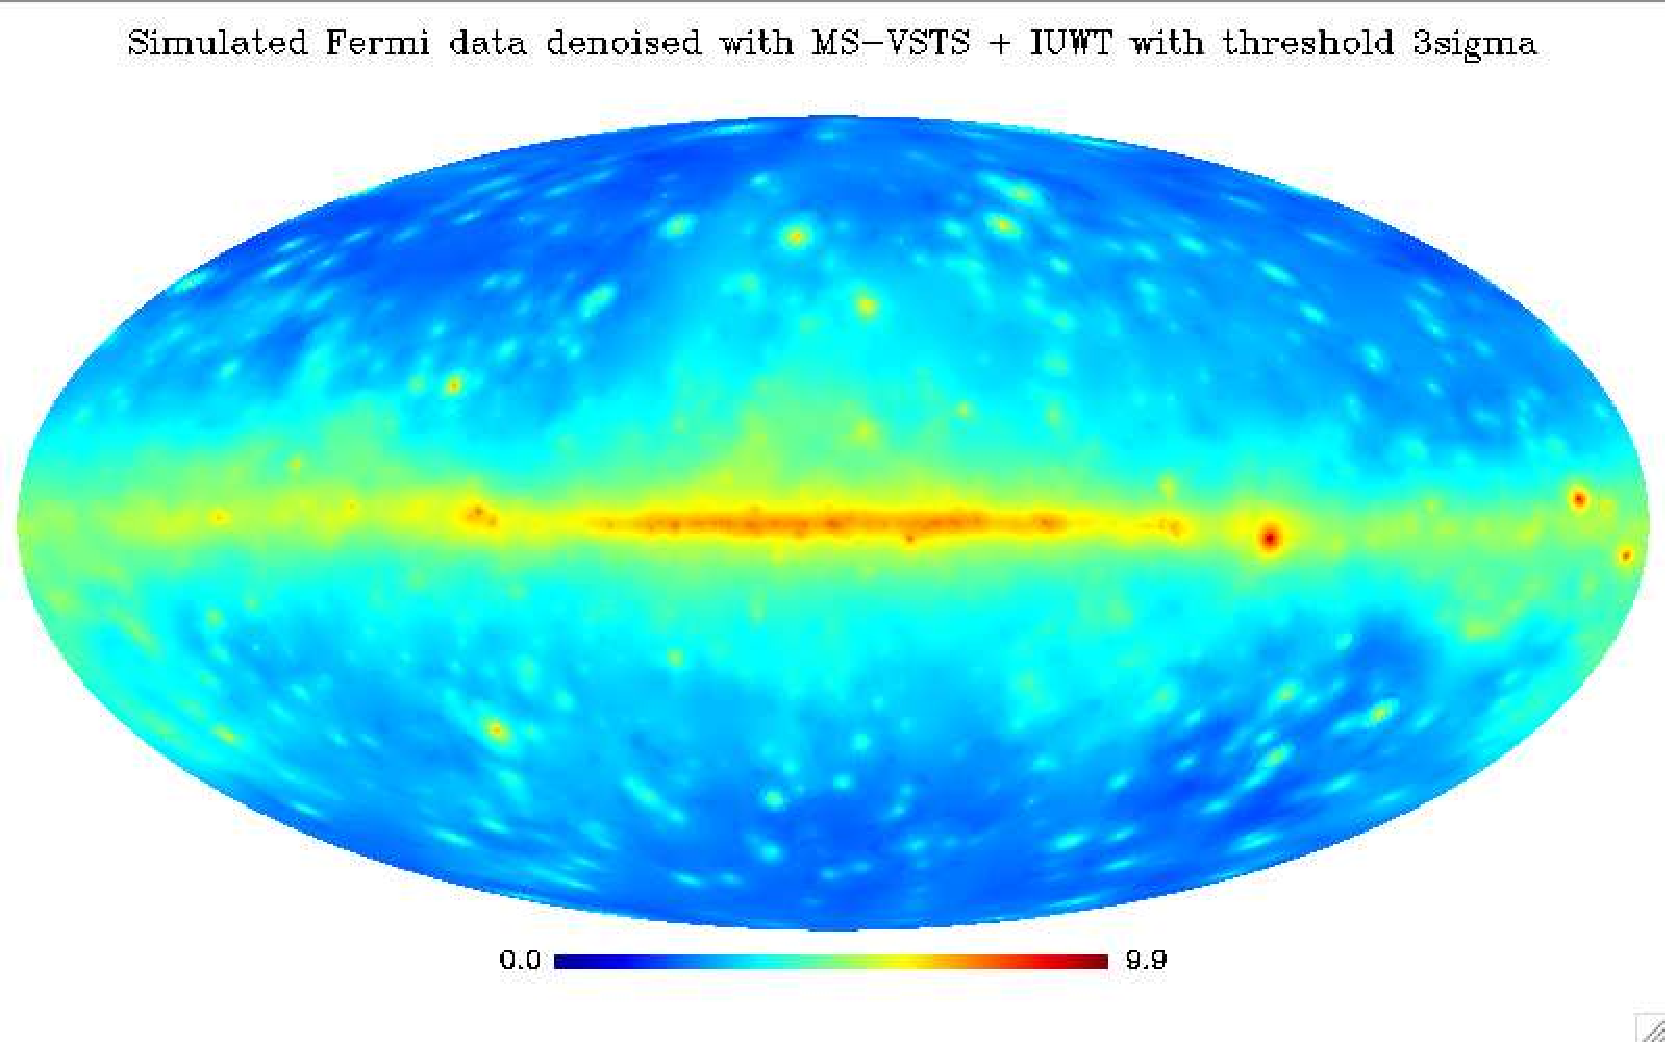
\includegraphics[width=3in,height=2.4in]{13822fg15.pdf}}

\caption{\emph{Top Left}: Fermi simulated map without noise.
\emph{Top Right}: Fermi simulated map with Poisson noise.
\emph{Middle Left}: Fermi simulated map denoised with Anscombe VST + wavelet shrinkage.
\emph{Middle Right}: Fermi simulated map denoised with MS-VSTS + curvelets (Algorithm~\ref{algcurv}).
\emph{Bottom Left}: Fermi simulated map denoised with MS-VSTS + IUWT (Algorithm~\ref{alg1}) with threshold $5\sigma_j$.
\emph{Bottom Right}: Fermi simulated map denoised with MS-VSTS + IUWT (Algorithm~\ref{alg1}) with threshold $3\sigma_j$.
Pictures are in logarithmic scale.}
\label{rechsd}
}
\end{figure}

\begin{figure*}
\begin{center}
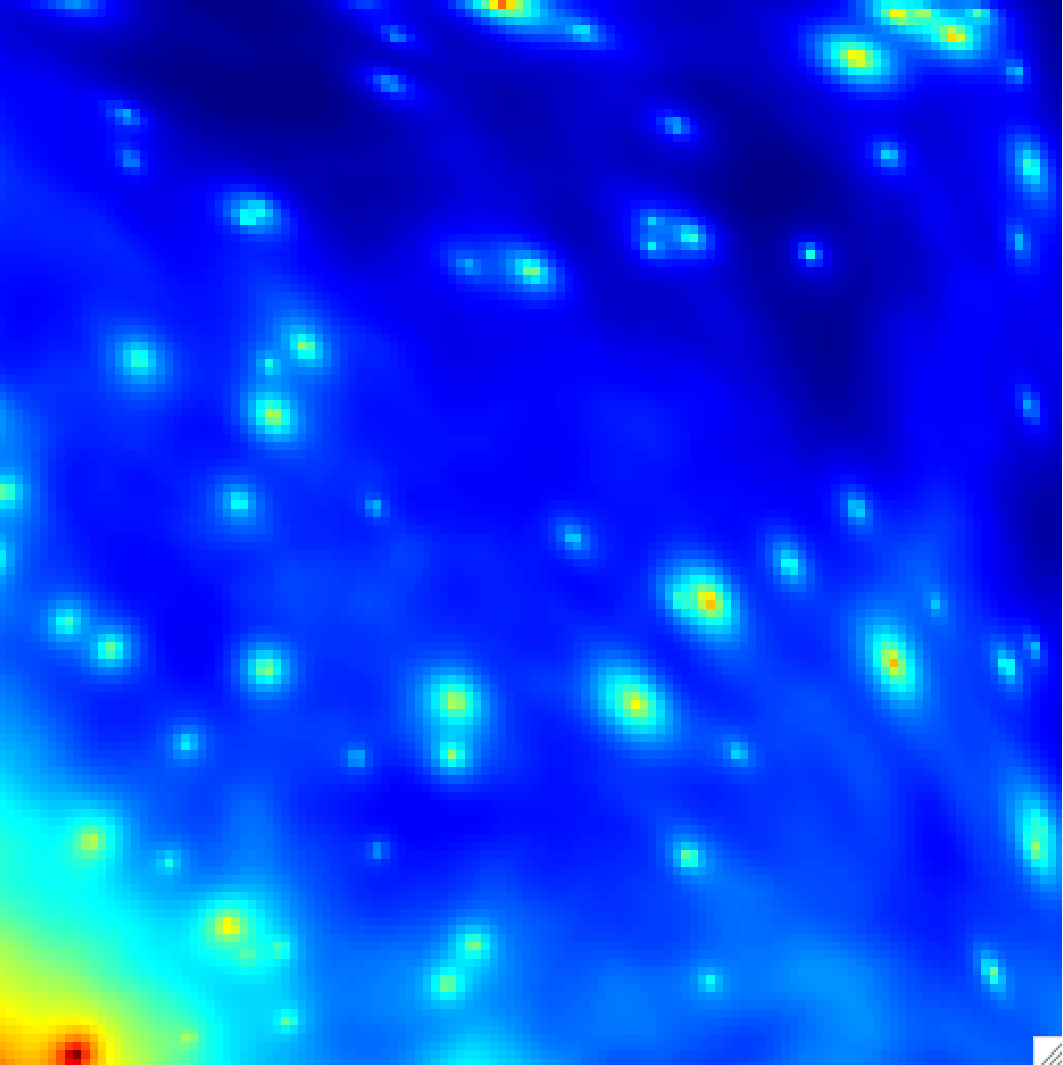
\includegraphics[width=2.5in]{13822fg16.pdf} \hfill
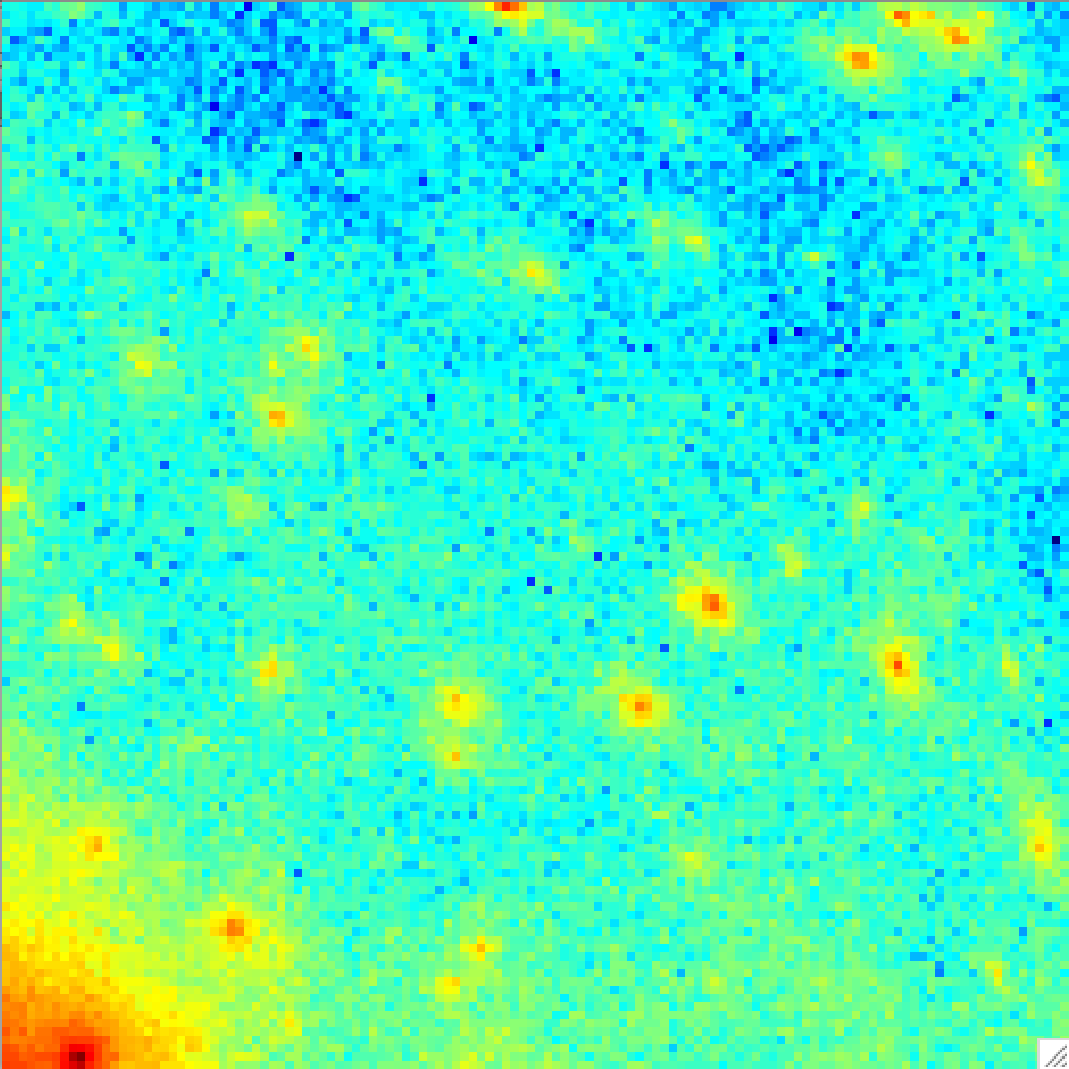
\includegraphics[width=2.5in]{13822fg17.pdf} \hfill
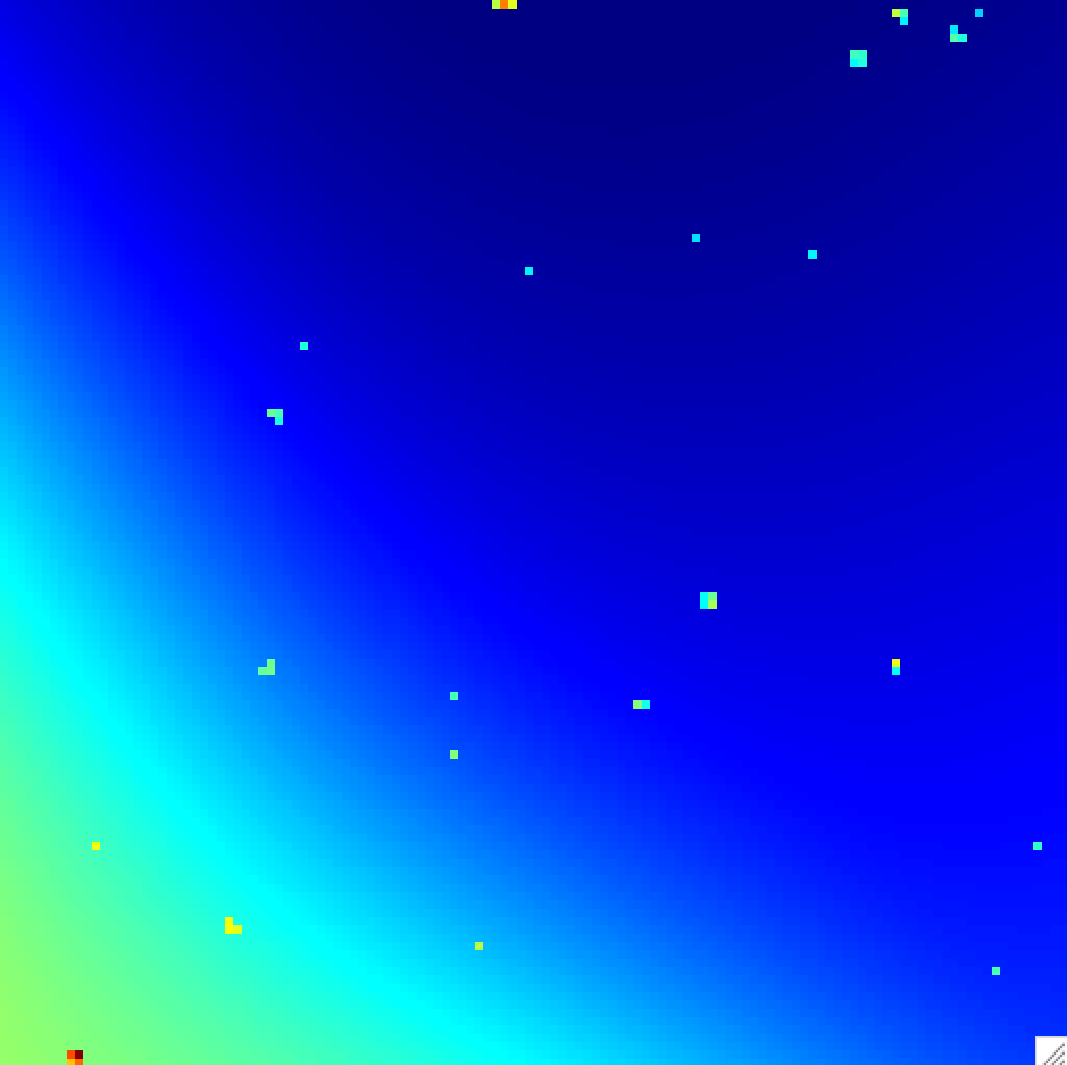
\includegraphics[width=2.5in]{13822fg18.pdf} \hfill
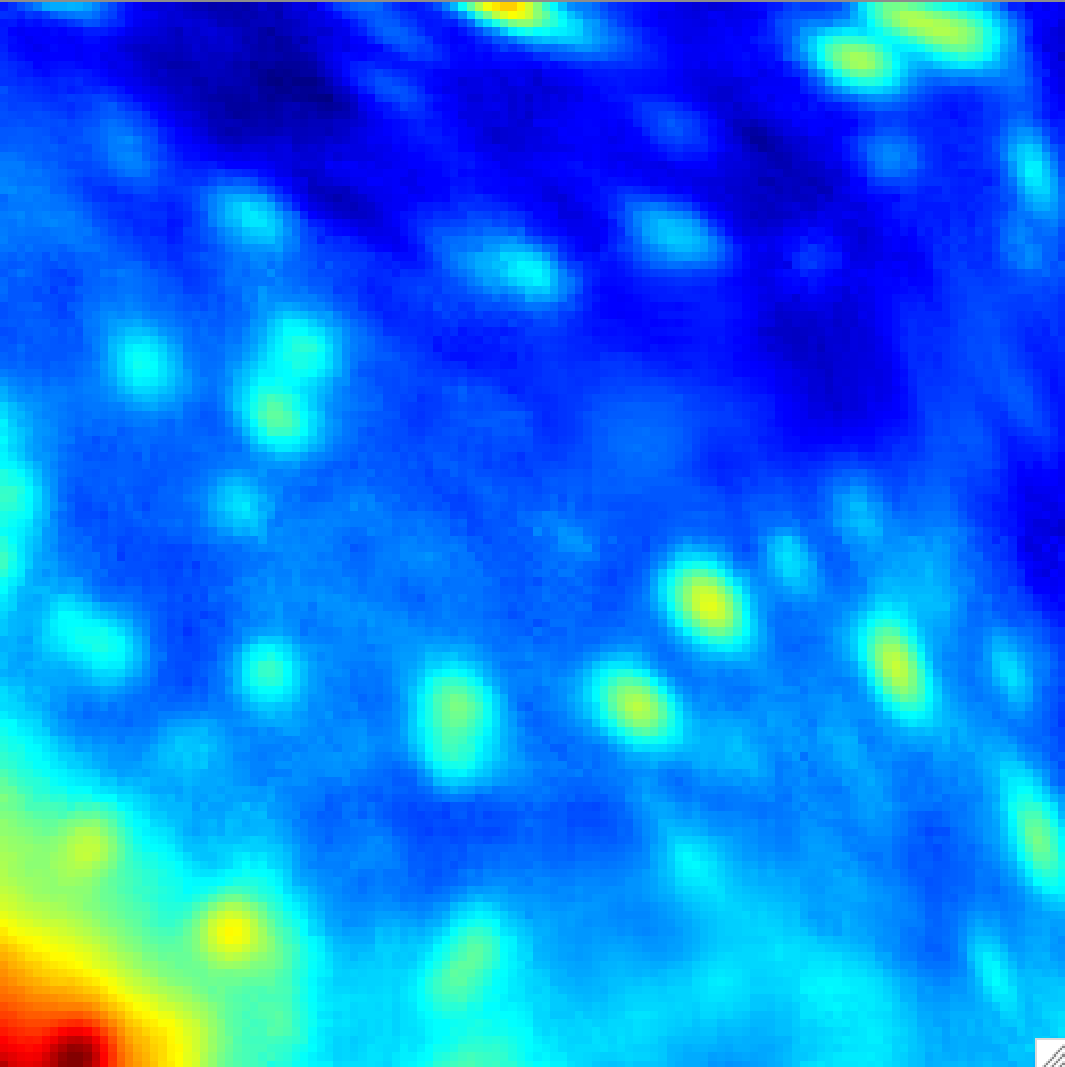
\includegraphics[width=2.5in]{13822fg19.pdf} \hfill
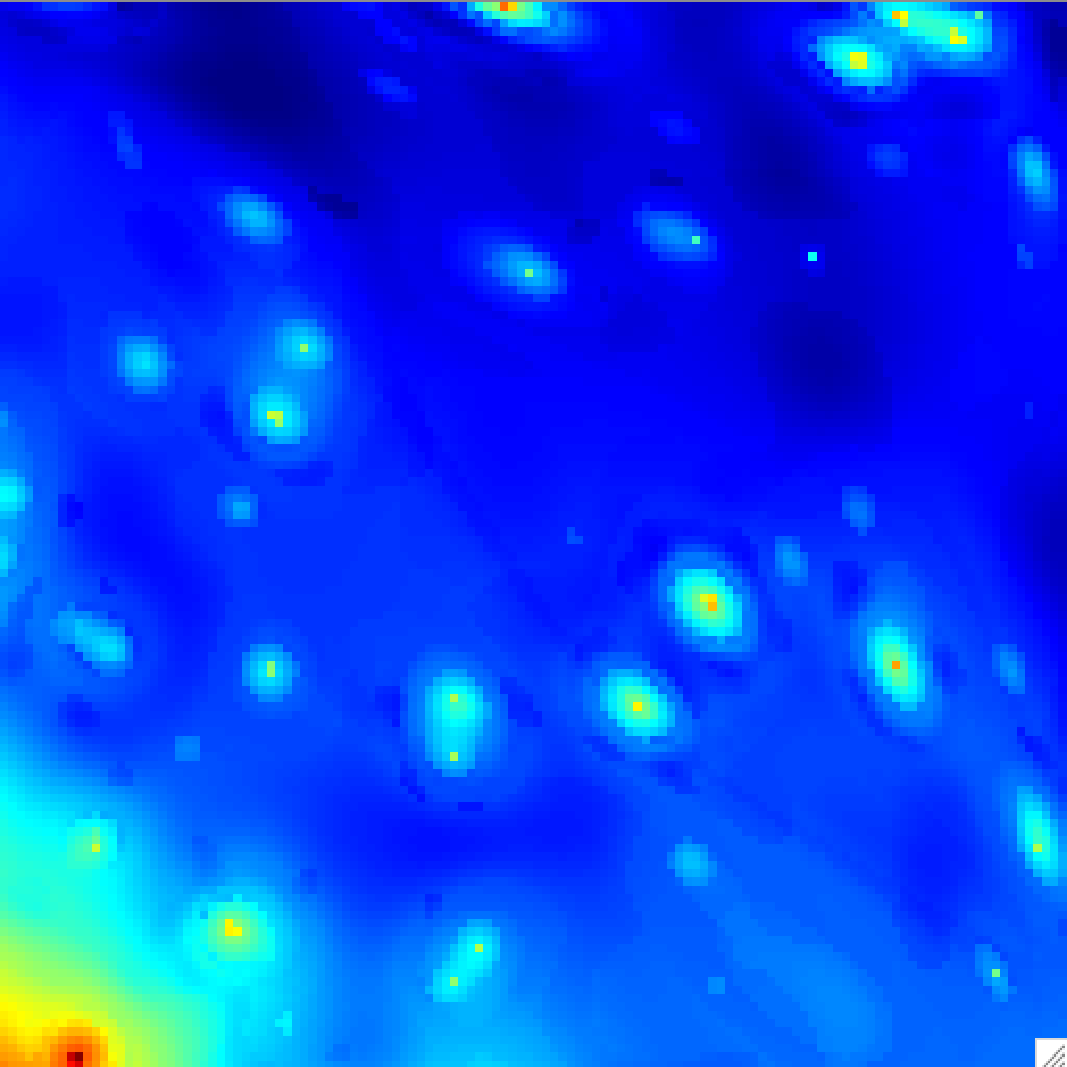
\includegraphics[width=2.5in]{13822fg20.pdf} \hfill
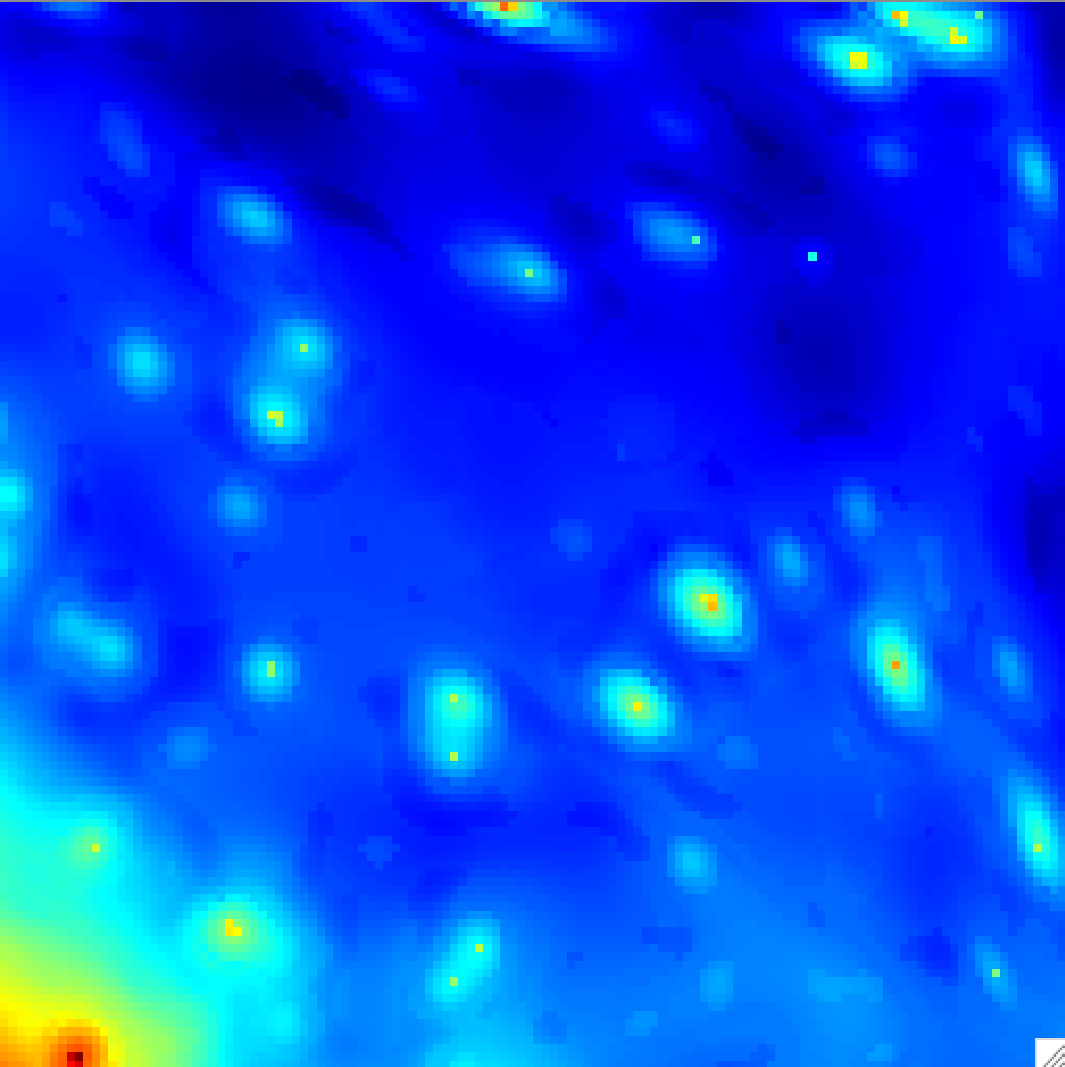
\includegraphics[width=2.5in]{13822fg21.pdf} \hfill
\caption{View of a single HEALPix face from the results of Figure~\ref{rechsd}.
\emph{Top Left}: Fermi simulated map without noise.
\emph{Top Right}: Fermi simulated map with Poisson noise.
\emph{Middle Left}: Fermi simulated map denoised with Anscombe VST + wavelet shrinkage.
\emph{Middle Right}: Fermi simulated map denoised with MS-VSTS + curvelets (Algorithm~\ref{algcurv}).
\emph{Bottom Left}: Fermi simulated map denoised with MS-VSTS + IUWT (Algorithm~\ref{alg1}) with threshold $5\sigma_j$.
\emph{Bottom Right}: Fermi simulated map denoised with MS-VSTS + IUWT (Algorithm~\ref{alg1}) with threshold $3\sigma_j$.
Pictures are in logarithmic scale.
}
\label{recface}
\end{center}
\end{figure*}
